\documentclass{beamer} 
\usepackage{beamerthemeTUM}
\usepackage[latin1]{inputenc} 
\usepackage{amsmath} 
\usepackage{amsfonts} 
\usepackage{amssymb} 
\usepackage{algorithm} 
\usepackage{algorithmicx} 
\usepackage[noend]{algpseudocode}
\usepackage{multicol} 
\usepackage{url}
\usepackage{graphics}
\usepackage{multicol}
\usepackage{eso-pic}
\usepackage{pst-node}
\usepackage{xcolor}
\usepackage{multido}
\usepackage{subfigure}
\usepackage{pstricks}
\usepackage{float} 

\graphicspath{{figures/}}

\setlang{en}


\author{Sebastian Lehnerer} 
\title{Multilabel Attribute Selection} 

\subtitle{cluster based group selection}
\email{lehnerer@in.tum.de}
\date{\today}
\institute[2011]{Technische Universit\"at M\"unchen}


\begin{document} 


\AddToShipoutPicture{\TitlePicture}
\maketitle
%\frame{\titlepage}
\ClearShipoutPicture
\AddToShipoutPicture{\BackgroundPicture}
\AtBeginPart{\frame{\partpage}}

\frame{
 {\insertsection} 
 \begin{itemize} 
  \item feature selection for each label
  \item using log-scores for further processing
  	\begin{eqnarray*} 
      Y_{1} &\leftarrow & \{X_{1}...X_{n} \cup Y_{1}...Y_{n}|X_{i},Y_{i}\in\mathbb R\}\\ 
      &\vdots &\\ 
      Y_{n} &\leftarrow & \{X_{1}...X_{n} \cup Y_{1}...Y_{n}|X_{i},Y_{i}\in\mathbb R\} 
    \end{eqnarray*} 
  	\item Hierachical Clustering using Chebyshev-, Euclidean-, Manhatten-, Mikowski-Distance
  	\item Single, Complete, Average and Mean Clustering
  	\item no. of clusters: $2,4,6$
  	 \end{itemize}
}

\frame{
 {\insertsection} 
 \begin{itemize} 
  \item \begin{scriptsize}
		\begin{algorithmic}
		   \Function{findLabelFeatureSets}{clusters}
			   	\State $ groups \gets Map<labelSet, featureSet> $
		   		\For{$ C \in clusters $} \Comment{every cluster}
		   			\State $currentLabelSet, currentFeatureSet $
		   			\For{ $ I \in C $ } \Comment{every instance}
						\For{ $ A \in I $ } \Comment{every attribute}
							\If{ $ score(A) > threshold $ }
								\If{ $ A \in labelSet $ }
									\State $ currentLabelSet \cap \{A\} $
								\Else
									\State $ currentFeatureSet \cap \{A\} $
								\EndIf
							\EndIf
		    			\EndFor
		    		\EndFor
		    		\State $ put(currentLabelSet, currentFeatureSet) \rightarrow groups $
		    	\EndFor
		    	\Return $groups$
		    \EndFunction
		  \end{algorithmic}
		\end{scriptsize}
	\end{itemize}
}

\frame{
 {\insertsection} 
		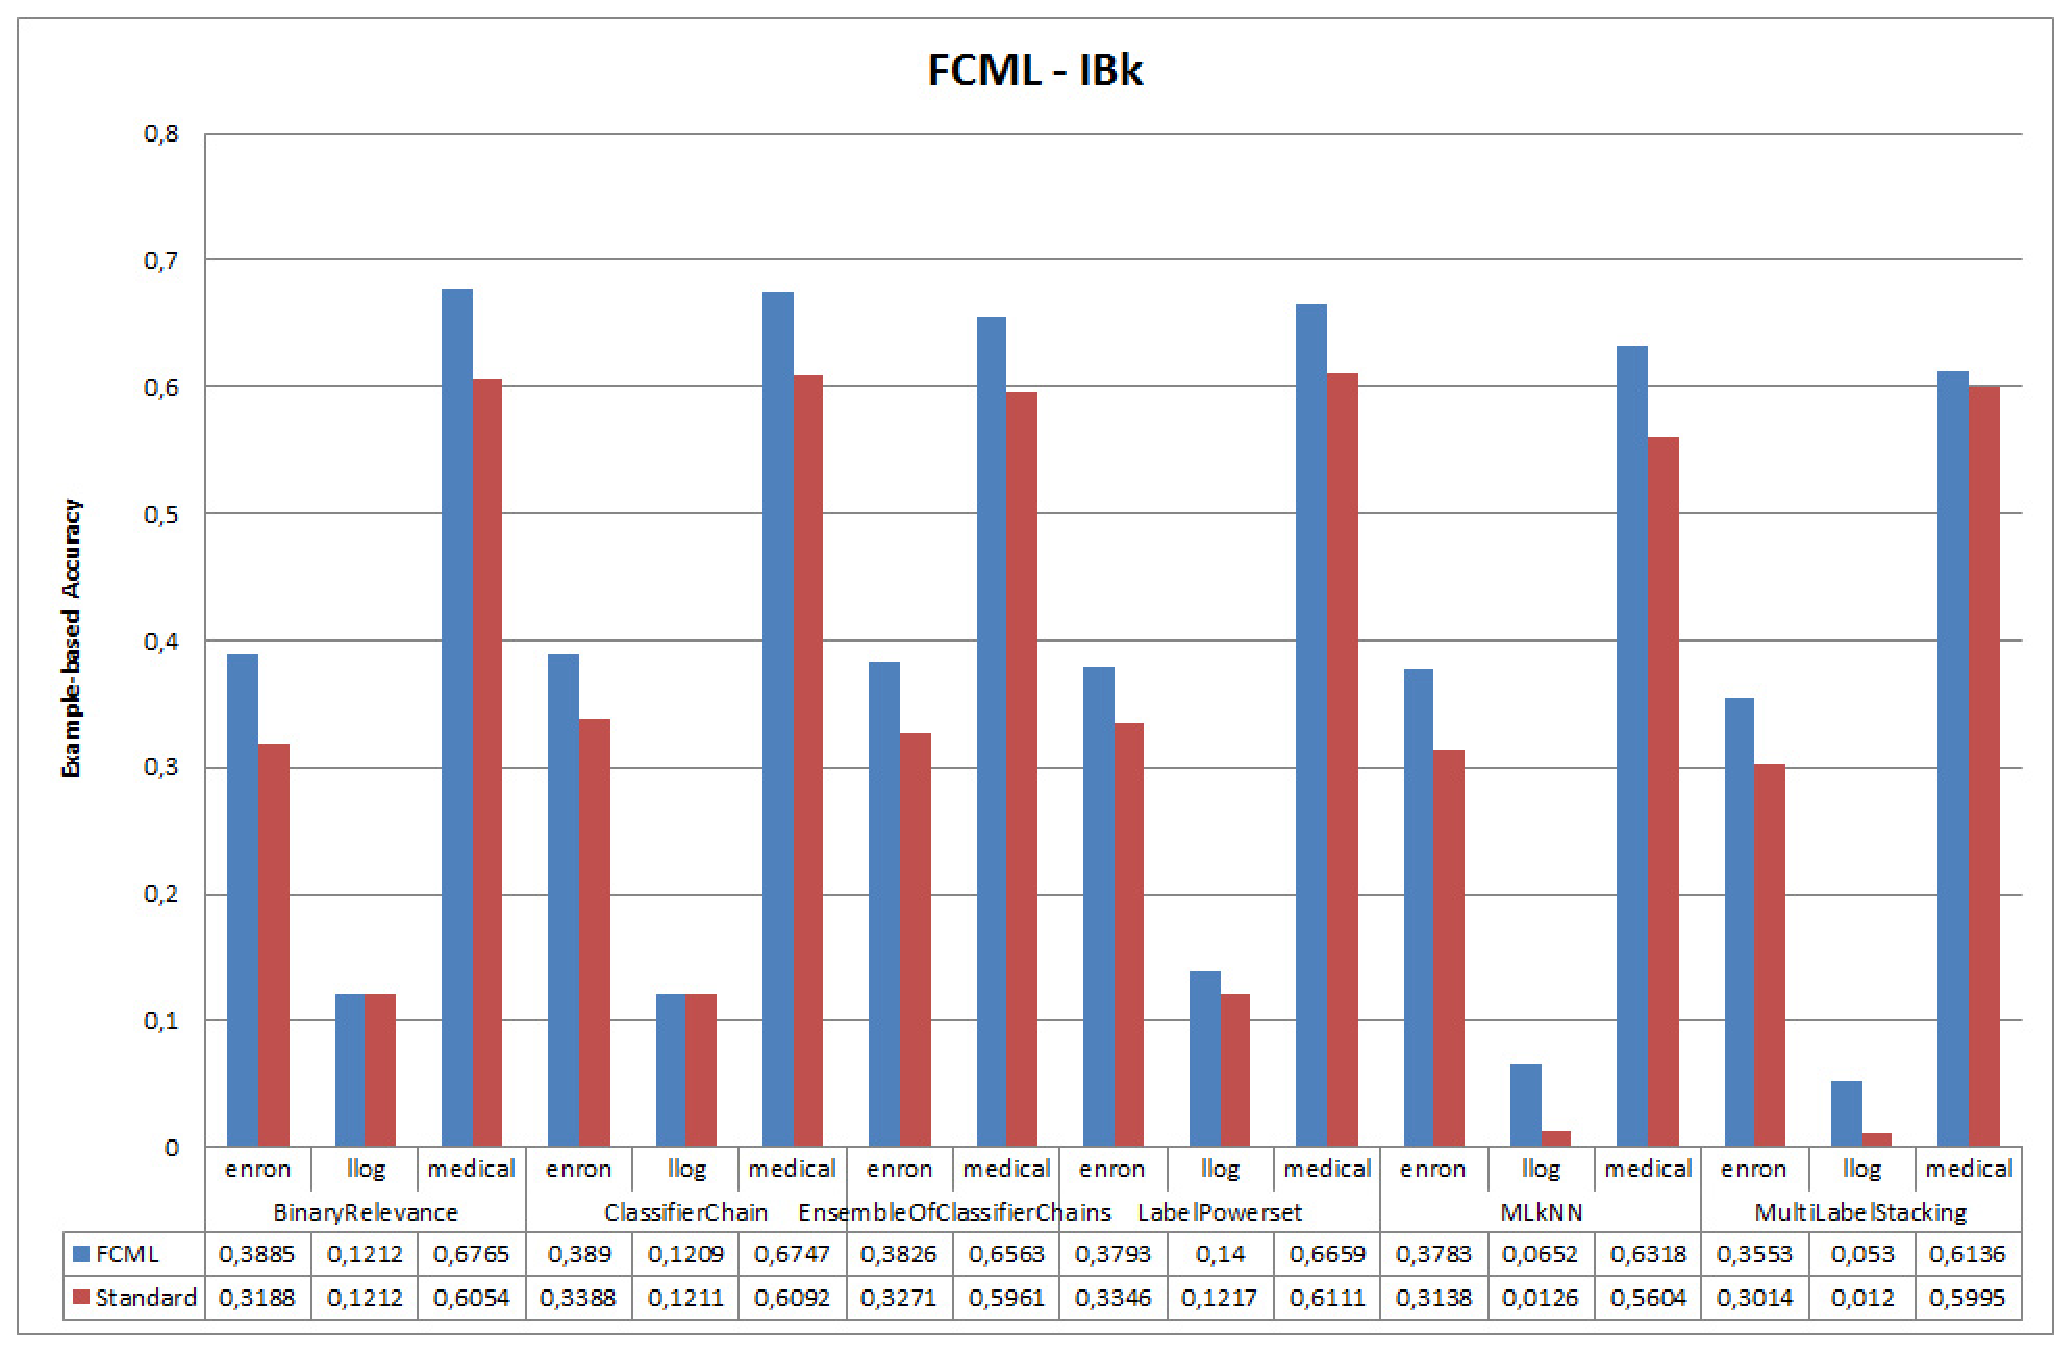
\includegraphics[scale=.3]{figures/fcml_results_ibk.eps} 
}


\frame{
 {\insertsection} 
		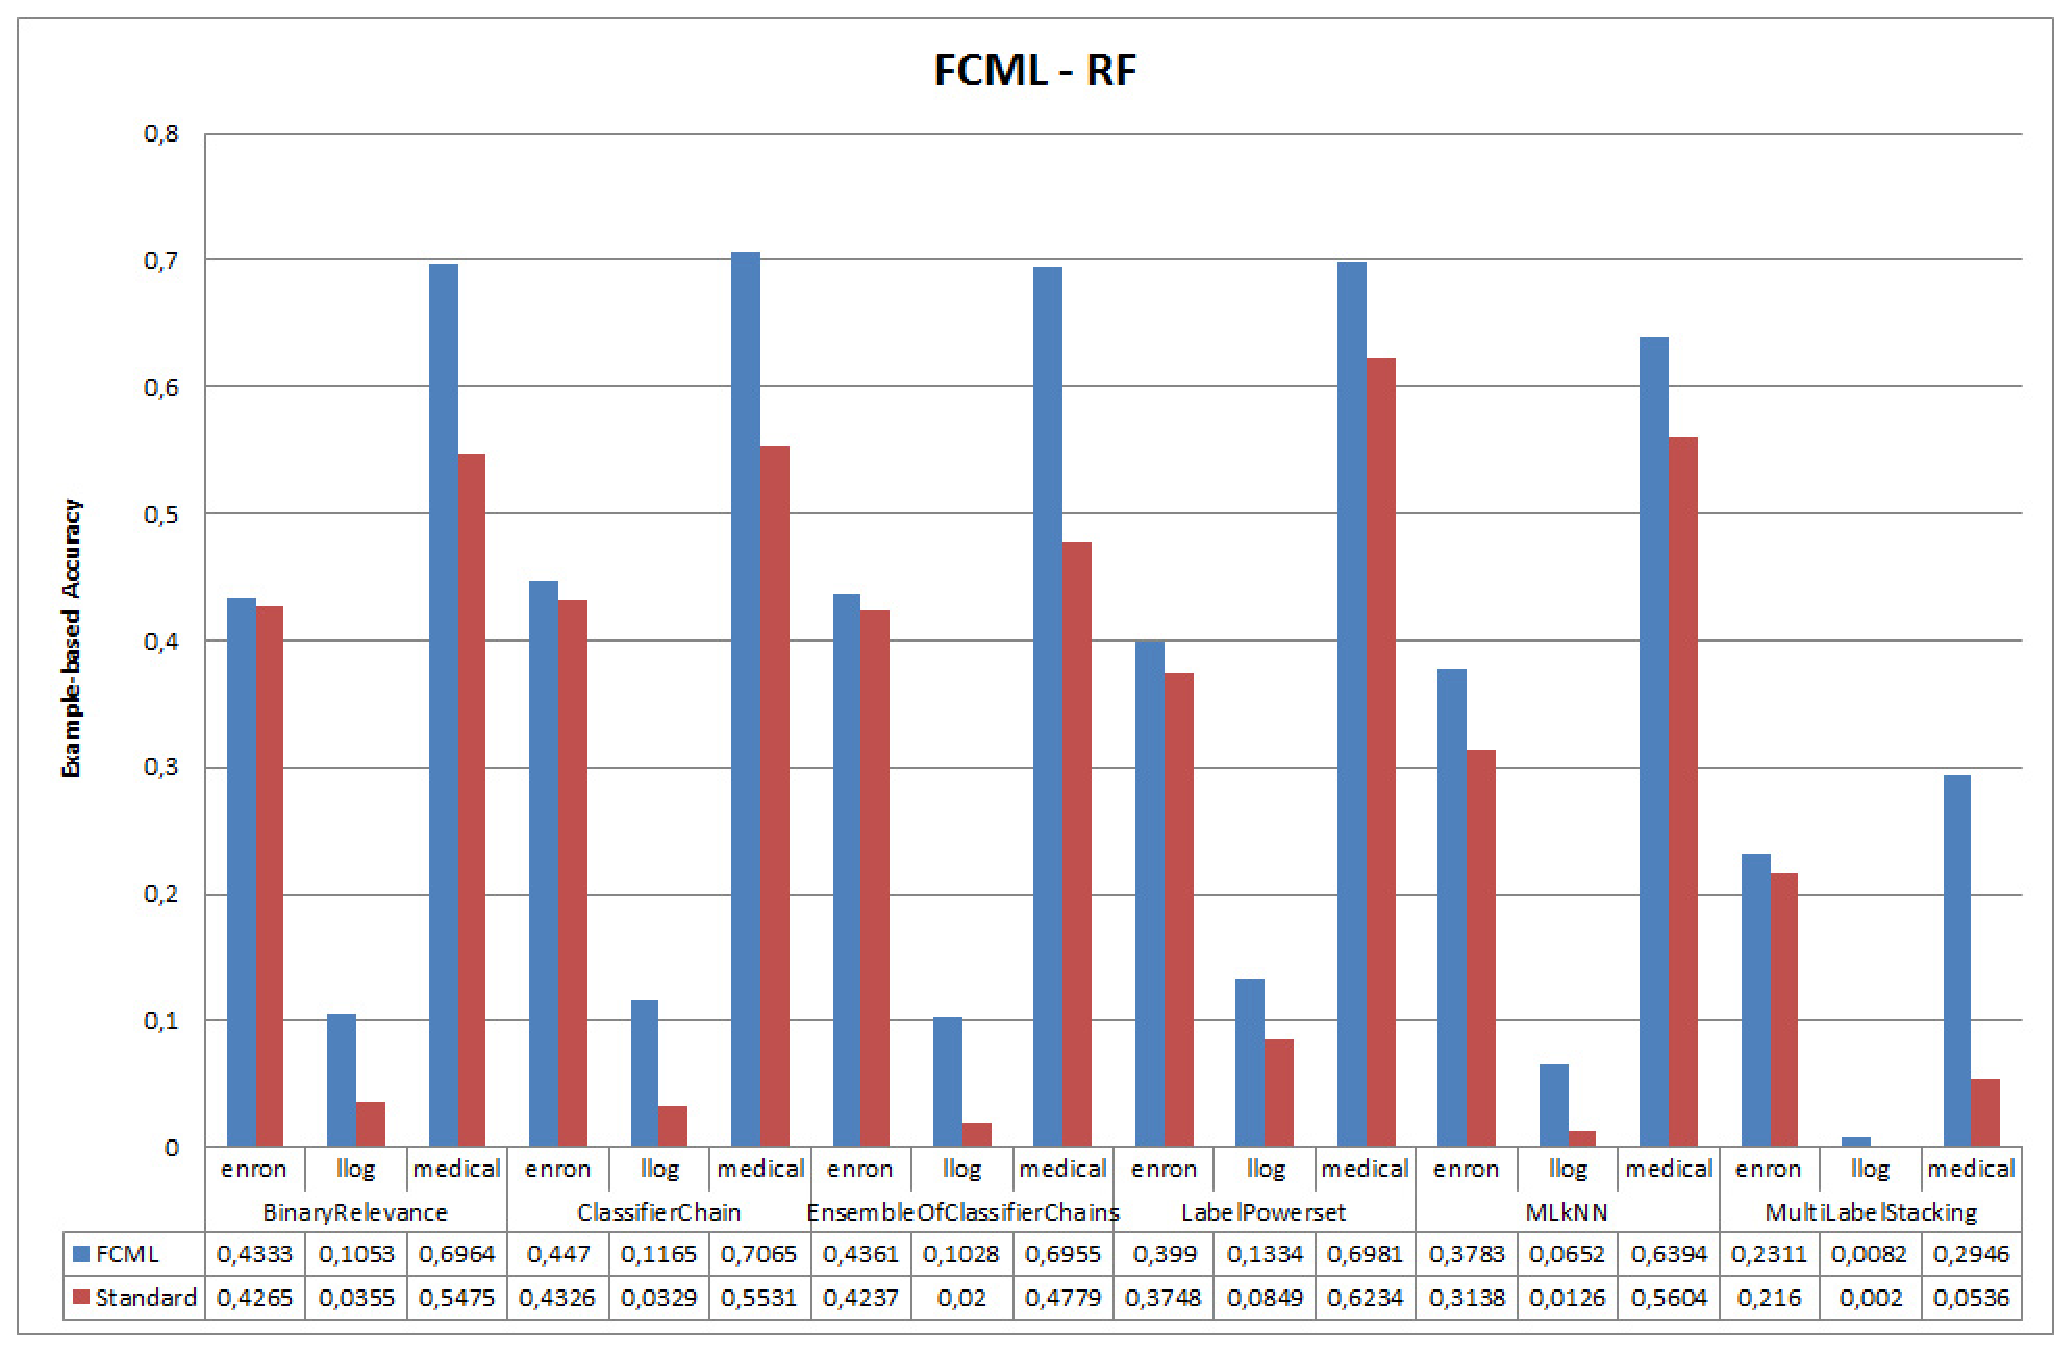
\includegraphics[scale=.3]{figures/fcml_results_rf.eps} 
}


\frame{
 {\insertsection} 
		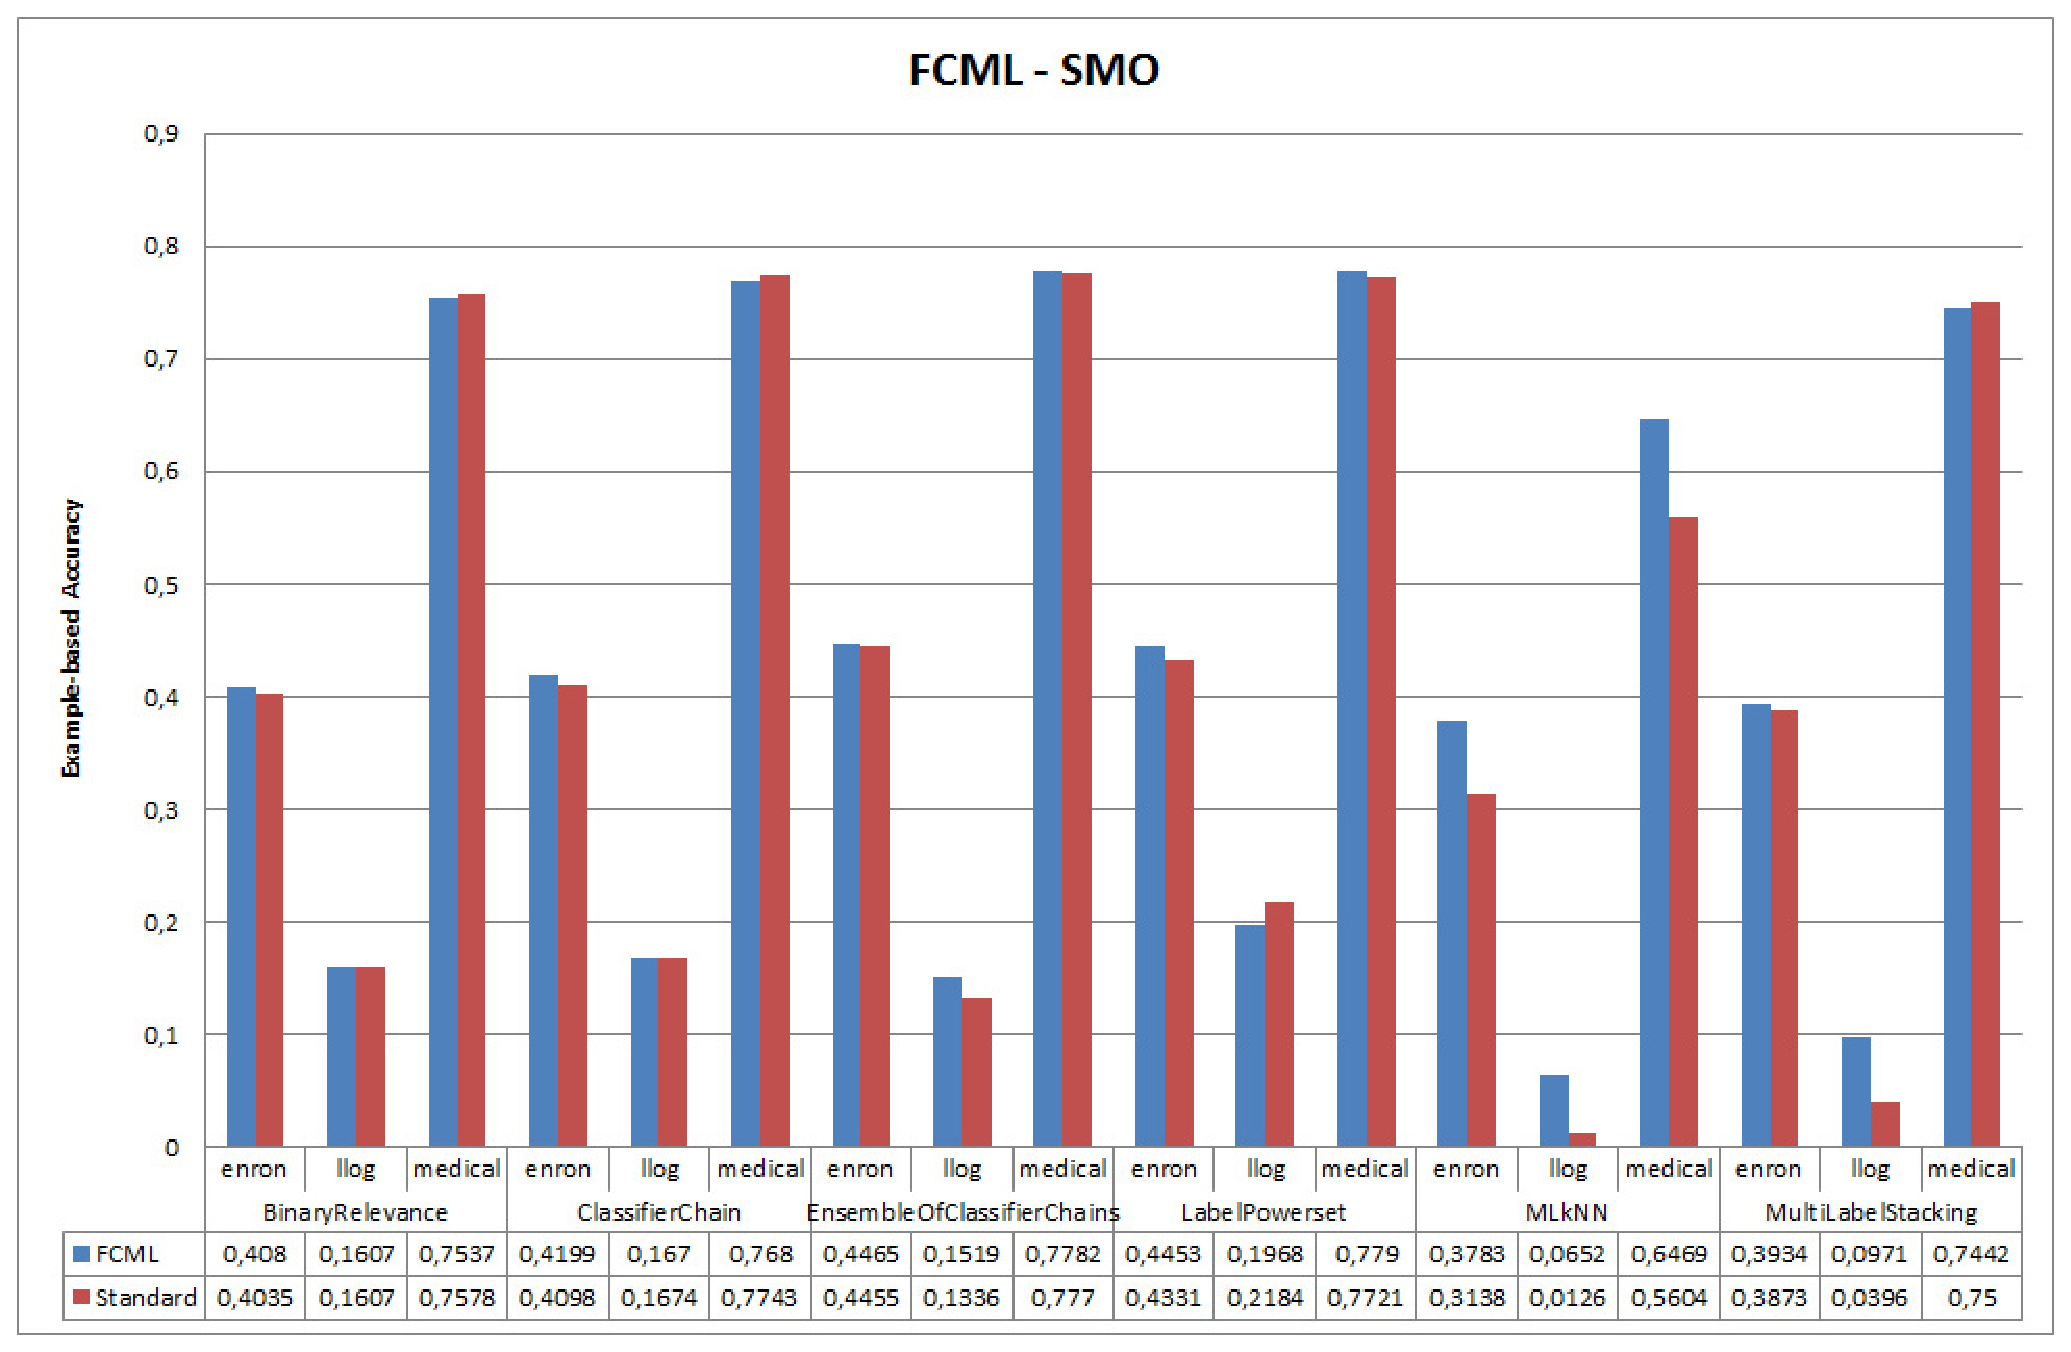
\includegraphics[scale=.3]{figures/fcml_results_smo.eps} 
}

\frame{
	{\insertsection}
	example cluster characteristics (\(\varnothing\) over folds)
	\scriptsize {
	\begin{itemize}
		\item enron\\
		\(\varnothing\) number of clusters : 2\\
		\(\varnothing\) number of cluster ($> 2$ labels) : 2\\
		\(\varnothing\) number of labels per cluster: 26.5
		\item llog\\
		\(\varnothing\) number of clusters :2 \\
		\(\varnothing\) number of cluster ($> 2$ labels) : 2\\
		\(\varnothing\) number of labels per cluster: 37.5	
		\item medical\\
		\(\varnothing\) number of clusters : 4\\
		\(\varnothing\) number of cluster ($> 2$ labels) : 1\\
		\(\varnothing\) number of labels per cluster: 11.25
	\end{itemize}
	}
}

\end{document}